\section*{Introduction}
This paper examines the incentives surrounding a particular program for allocating public infrastructure funds. It determines if the program incentivizes clientelistic spending or spending allocated to benefit incumbent politician supporters.
To investigate clientelistic spending in politics, we exploit a program known as the Aldermanic Menu Program in the City of Chicago. 
The aldermanic menu program was initiated in 1994 and continues to this day \cite{OIGaudit}. 
The program delegates approximately \$ 66 million every year to be split equally amongst the 50 aldermen in Chicago's city council to be spent on projects they unilaterally select for their ward, given a ``menu'' of acceptable expenditures. 
However, ``off-menu'' expenditures are also allowed, of which most ``off-menu'' funds go towards Parks, Chicago Public Schools, and miscellaneous beautification projects such as trees, murals, decorative garbage cans, designer bike racks, and more\cite{OIGaudit}. 
While on-menu items are typically also provided by other funding sources within Chicago's Capital Improvement Program, off-menu items such as murals and statues are usually directly credited to the Aldermen, thus giving an incentive to reward supporters' loyalty with public goods.
The program is unique insofar as it gives elected politicians a wide berth over a significant portion of the City's infrastructure budget and allows its use for items one does not typically think of as core infrastructure. 
An example of a portion of a menu from 2013 is shown below in Figure~\ref*{fig:menu_example}.


\begin{figure}[H]
    \centering
    \caption{An Example of an Aldermanic Menu from 2012/2013}\label{fig:menu_example}
    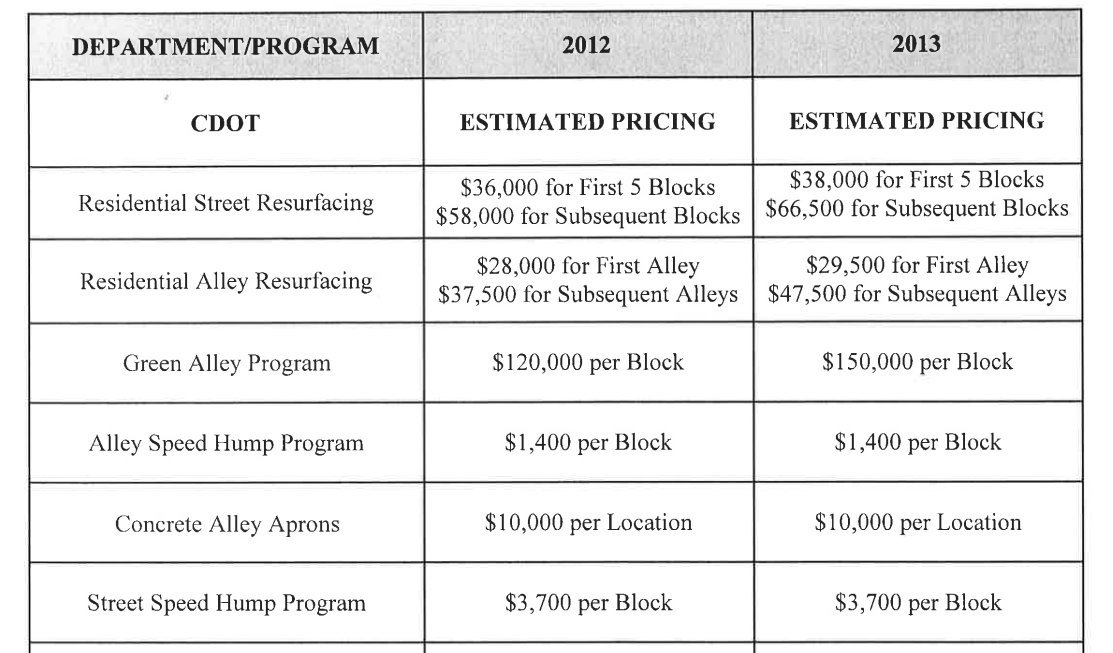
\includegraphics[scale=0.38]{input/menu_example.png}
\end{figure}

The Chicago Office of the Inspector General audited the program in 2017 and found that the program was rife with misallocation -- since wards are defined to be approximately equal by population but not equal by area, so wards with a larger area have more infrastructure to maintain \cite{OIGaudit}.
Thus, the OIG found that the program resulted in significant funding disparities between wards relative to infrastructure needs.
Secondly, the OIG audit found that from 2012 through 2015, the program permitted aldermen to use \$ 15.1 million in menu funds for projects unrelated to so-called ``core'' infrastructure.
Finally, the OIG audit found that CDOT allowed aldermen to use \$825,292 of menu funds on projects outside of the ward they were elected to represent so that they could spend it on the wards they were running for reelection in.

In this paper, we examine how political incentives distort the allocation of public goods in Chicago's Aldermanic Menu Program.
In doing so, we make two main contributions.
First, we find that ``menu''-style programs allow entrenched politicians to form clientelistic relationships with their constituents, evidenced by a case study and a differences-in-differences design focusing on entrenched, corrupt aldermen.
Second, we find that this relationship is mitigated by electoral competition, as these effects go away when we focus on incumbents removed by close elections. 
Thus, this provides evidence that electoral competition can mitigate clientelism and that policies expanding ease of entry into politics can reduce patronage.

Section 2 of this paper describes the dataset collected for this paper. 
It first goes through the data collection process, then describes summary statistics of the data itself, and displays a map of total spending distribution.
Section 3 describes the case study of Alderman Bernie Stone, who was long-rumored to have used the program selectively on his supporters.
We document evidence for this by looking at how spending shares changed after challenger Debra Silverstein defeated him in 2011. 
Before Stone was defeated, we find that he allocated almost no menu funds to the bottom 20\% of precincts by campaign contribution. 
After he was defeated by Debra Silverstein, the bottom 20\% of precincts by campaign contribution each received 1.77\% more of the menu funds than they did before Stone was defeated.
In total, this constitutes a difference of \$ 20,000 per year compared to the average spending per precinct of \$ 23,636 per year. 
Section 4 explains this paper's empirical strategy to determine if the Stone case study can be generalized to other aldermen.
Section 5 shows the results of said empirical strategy, which finds that Aldermen removed or retired due to criminal indictments, which has similar results to the Stone case study. 
However, this does not generalize to competitive elections.
The results from the indictment-based differences-in-differences design are statistically weak and sensitive to the number of precincts included, but the economic magnitude is not. 
Section 6 concludes and discusses the implications of this paper.

This paper is deeply related to the literature on how politicians allocate public funds. Still, relatively few cases exist where an elected official gets direct, personal control over budget allocations. 
The cases in the literature are much more common, where politicians have indirect control over public spending via voting in governing bodies.
An example of this kind of study is \cite{levitt1997impact}, where Levitt found that US congresspeople who can get more funds allocated to their constituents tend to win more votes. 
Levitt estimated this via an IV approach that exploited expenditures to areas outside the congressperson's district but within the same state to disentangle the reverse causality between reelection probabilities and political allocations. 

Then there is \cite{finan2021electoral}'s study that looks at the allocation of funds from Brazil's federal legislature, where similarly, each of the 513 legislators in Brazil receives a fixed budget of BRL\$1.5 million each year for similar public infrastructure projects.  
Furthermore, electoral competition in Brazil is intense: Only 75\% of legislators choose to run for reelection compared to Chicago's city council reelection rate of 87\%.
Furthermore, incumbents can be challenged by other incumbents due to overlapping districts, whereas in Chicago, this problem only rarely happens when wards are redrawn.
In this paper, Finan and Mazzocco estimate a structural model to find that 26\% % of public funds are distorted relative to a social planner's allocation. 
After estimating their structural model, they also found that implementing an approval voting system would reduce the distortions by 7.5\%. 
They also find that term limits may reduce distortion but increase corruption.

Most of the literature on pandering from public economics focuses intently on theoretical models to explain behavior but comparatively little empirical testing of that behavior. 
This literature on pandering looks primarily at the incentives to pander, noting such studies as \cite{MASKIN201979},  and \cite{ENIKOLOPOV201474}. 
The Maskin and Tirole study focuses instead on pandering, defined as targeting spending towards interest groups to signal that politicians share their concerns.
They find that pandering increases spending in accountable officials if either official's overall spending propensity is known. 
Enikolopov, on the other hand, is a more empirical study that shows that elected politicians are more prone to targeted redistribution efforts than appointed public officials and builds a model consistent with that concept by focusing on patronage jobs in local government. 
Enikolopov shows that the number of public employees is pro-cyclical with the election cycle, where the number of public employees increases in election years and decreases in off-election years. 
Finally, they show that older, non-elected officials increase hiring. 
They claim this is because younger non-elected officials have more substantial career concerns.

However, this study borrows the most from the \cite{fowleretalquidproquo} study, which uses a combination of regression discontinuity and first-differences design to study whether there is evidence of successful corporate campaign contributions influencing the stock prices of the donors. 
From this two-pronged approach, Fowler et al. found that there really is no impact of a preferred candidate on winning, and thus, it is hard to argue that campaign contributions are a profitable venture for companies. 
We will use a similar two-pronged approach to determine if newer politicians are more likely to spend conspicuously than experienced politicians. 

In addition, this study is different from traditional political economy studies as it focuses on a municipal environment. 
Thus, it is also related to the literature on municipal infrastructure provision and the new quantitative spatial economics literature.
This includes \cite{Glaeser2018political}, \cite{Fajgelbaum2023}, \cite{treb_arkolakis_2022_infrastructure}, and \cite{bordeu2023commuting}.
Glaeser's seminal paper focuses on infrastructure's ``visible'' and ``invisible'' effects. 
In particular, he finds that governments spend too much on new infrastructure projects and not enough on maintenance.
Furthermore, local voters are less likely to support new projects due to noise, land use, and other externalities from new construction.
Glaeser uses this framework to explain the decline of urban mega-projects.
Our framework differs as we look at the allocation of relatively low-nuisance maintenance and public goods projects rather than new construction.
Thus, we see the opposite problem in maintenance: electoral concerns lead to too much spending on supporters and not enough on the rest of the municipality.
Fajgelbaum et al. examine how political economy influenced the planning of California's high-speed rail (CHSR) project.
They find that preferences for widespread approval lead to the planner placing CHSR stations farther from dense metro areas than a politically blind planner.
Treb and Arkolakis' paper uses a quantitative spatial model to evaluate the impact of improving any segment of the infrastructure network on the entire network's welfare, and finds in an empirical application that there are highly variable returns to investment across different links in the network.
Finally, Bordeu looks at how infrastrucuture is allocated across a similarly decentralized city, Santiago, Chile, and finds that the sub-city municipalities over-invest in core areas and under-invest in areas near their boundary using a quantitative spatial model.
This results in higher-cross-jurisdiction commuting costs, less concentrated employment, and a wider spatial distribution of production.
She finds that infrastructure centralization would increase aggregates infrastructure investment and population and yields large welfare gains.
